\section{Modélisation du comportement mécanique de la tête de coupe}
\begin{obj}
Modéliser le comportement dynamique de la tête de coupe afin d’identifier un phénomène de vibration néfaste au regard de l’exigence 1.2.2.
\end{obj}

\subsection*{Modélisation du comportement cinématique de la tête de coupe}
\begin{obj}
Déterminer la loi entrée/sortie de la chaîne cinématique de la tête de coupe et valider son comportement vis-à-vis des exigences 1.2.2.3 et 1.2.2.4.
\end{obj}

La découpe du tissu est réalisée par un mouvement de translation alternative d’une lame par rapport au matelas de tissus. Ce mouvement est obtenu par un système bielle-manivelle dont le schéma cinématique est donné par la figure 9. Les mouvements de translation de la tête de coupe par rapport à la table impliquent que les bases $\base{x_2}{y_2}{z_2}$ et $\base{x_0}{y_0}{z_0}$, liées respectivement à la tête de coupe et à la table, sont identiques (figure \ref{fig_01}).


\begin{figure}[!h]
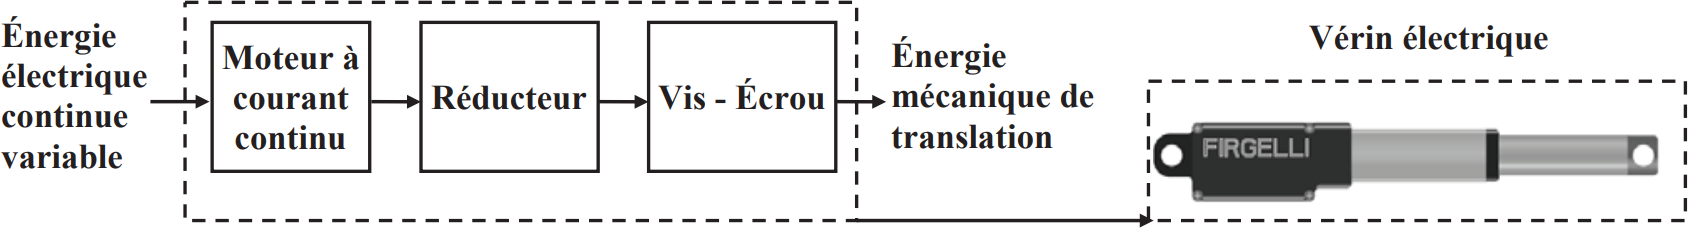
\includegraphics[width=\linewidth]{fig_09.png}
\caption{Système d’entraînement de la lame de coupe et schéma cinématique associé\label{fig_09}}
\end{figure}

\paragraph*{Modélisation des liaisons et paramétrage du système}

On associe le repère  $\rep{2}=\repere{A}{x_2}{y_2}{z_2}$ à la tête 2, le repère $\rep{3}=\repere{A}{x_3}{y_3}{z_3}$ à la manivelle 3, le repère $\rep{4}=\repere{B}{x_4}{y_4}{z_4}$ à la bielle 4 et le repère $\rep{5}=\repere{C}{x_5}{y_5}{z_5}$ à la lame 5.

La manivelle 3 est en liaison pivot avec la tête 2, d’axe $\axe{A}{y_2}$ et d’angle $\theta_{32} (t)= \angl{x_2}{x_3} = \angl{z_2}{z_3} $.

La manivelle 3 est en liaison pivot avec la bielle 4, d’axe $\axe{B}{y_2}$ et d’angle $\theta_{43} (t)= \angl{x_3}{x_4} = \angl{z_3}{z_5} $.

La bielle 4 est en liaison pivot avec la lame 5, d’axe $\axe{C}{y_0}$ et d’angle $\theta_{54} (t)= \angl{x_4}{x_2} = \angl{z_4}{z_2} $.

La lame 5 est en liaison glissière avec la tête 2, de direction  $\vz{2}$ et de paramètre linéaire $\lambda(t)$.
On pose $\omega_{ij} (t)= \dfrac{\dd \theta_{ij}}{\dd t} = \thetap_{ij}(t)$, $\vect{AB}=L_3\vz{3}$ avec $L_3=\SI{12,5}{mm}$, $\vect{BC}=L_4 \vect{z_4}$  avec $L_4=\SI{80}{mm}$ et $\vect{AC}=\lambda(t)\vz{2}$.

\begin{marginfigure}
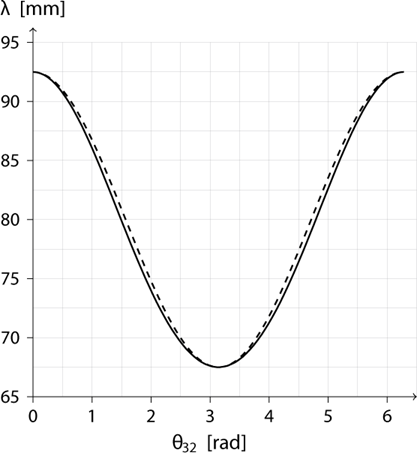
\includegraphics[width=\linewidth]{fig_10}
\caption{ Évolutions théorique ( -- ) et approximée ( - - ) du paramètre $\lambda$ \label{fig_10}}
\end{marginfigure}

\begin{marginfigure}
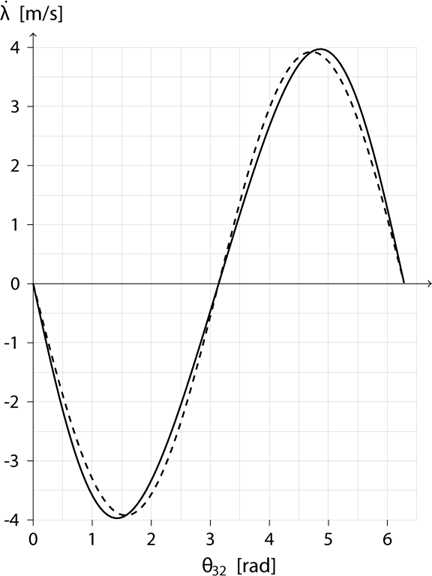
\includegraphics[width=\linewidth]{fig_11}
\caption{ Évolutions théorique ( -- ) et approximée ( - - ) de la vitesse $\lambdap$ pour une vitesse $\thetap_{32}=\SI{3000}{tr/min}$ \label{fig_11}}
\end{marginfigure}

\question{Déterminer la relation entre le paramètre $\lambda(t)$, l’angle $\theta_{32} (t)$ et les données géométriques du système.}

\question{En déduire l’expression littérale de l’amplitude des oscillations de la lame, notée $\Delta z$. Faire l’application numérique et conclure sur le respect de l’exigence 1.2.2.3.}

\question{Donner les hypothèses permettant de montrer que la loi obtenue précédemment peut se mettre sous la forme $\lambda(t)\simeq L_3 \cos \left(\theta_{32}(t)\right)+L_4(t)$.}% $\lambda(t) \simeq L_3 \cos⁡\left(\theta_{32}(t)\right) + L_4(t)$.}

Afin de valider cette approximation, les deux fonctions mathématiques ont été tracées sur un tour de l’arbre moteur (figure \ref{fig_10}).




\question{Conclure sur l’adoption de la loi approximée dans la suite de l’étude.}

Afin de valider le critère associé à l’exigence de vitesse de coupe, il est nécessaire de déterminer la loi en vitesse de la lame notée $\lambdap(t)$.

\question{Déterminer l’expression littérale de $\lambdap(t)$ à partir du modèle simplifié de $\lambda(t)$. }

Cette loi en vitesse simplifiée a été tracée (figure \ref{fig_11}) pour être comparée à la loi obtenue à partir du modèle établi initialement.

\question{La simplification de la loi en vitesse permet-elle de valider l’exigence 1.2.2.4. ?}
